\section{Motivation}
A polynomial can be represented in various ways. Each representation has its advantages and downsides.

In general, a polynomial $A(x)$ of degree $n-1$ can be written as
$$
\begin{aligned}
    A(x) &= a_0 + a_1x + a_2x^2 + \cdots + a_{n-1}x^{n-1} \\
    &= \sum_{k=0}^{n-1} a_k x^k
\end{aligned}
$$

\subsection{Coefficient Vector}

For a polynomial $A(x)$ of degree $n-1$, the coefficient vector contains the coefficient of the polynomial represented as a vector.
$$
A(x) = a_0 + a_1 x + a_2 x^2 + \cdots + a_{n-1}x^{n-1} \quad  \leftrightarrow \quad \langle a_0,a_1,a_2,\ldots,a_{n-1} \rangle
$$

\subsection{Roots}

Equivalently,
$$
A(x) = (x-r_0) (x-r_1) \cdots (x - r_{n-1}) \cdot c
$$
where $r_0,r_1,\ldots,r_{n-1}$ are the $n$ roots of the polynomial and $c$ is a scale term.

\subsection{Samples}

Given a polynomial, we can take $n$ points (coordinates): 
$$
(x_0,y_0),\, (x_1,y_1),\, \ldots ,\, (x_{n-1},y_{n-1})
$$
where $A(x_i)=y_i$ for all $i \in \{0,1,\ldots,n-1\}$. This representation is also known as the point-value representation.

By the Foundamental Theorem of Algebra, these samples uniquely define a polynomial of degree $n-1$.

\begin{theorem}[The Fundamental Theorem of Algebra]
    A univariate polynomial of degree $n$ with complex coefficients has exactly $n$ complex roots.
\end{theorem}

\begin{corollary}[Uniqueness of Polynomial Interpolation]
    A degree $n-1$ univariate polynomial $A(x)$ is uniquely defined by its evaluation at $n$ distinct values of $x$.
\end{corollary}

\section{Operations on Polynomials}

There are three primary operations on polynomials: evaluation, addition, and multiplication. The complexity of these operations varies depending on the representation. There is not a single representation that is efficient for all operations, so we need a way to efficiently convert between the representations. 

\subsection{Coefficient Representation}

\subsubsection{Evaluation}

Evaluation is efficient when the polynomial is represented as the coefficient vector using the Horner's rule:
$$
A(x_0) = a_0 + x_0 (a_0 + x_0 (a_2 + \cdots + x_0 (a_{n-2} + x_0 (a_{n-1})) \cdots ))
$$
which can be written in pseudocode as follows
\begin{codebox}
    \Procname{$\proc{Evaluate}(A=\langle a_0,\ldots a_{n-1}\rangle,\,x)$}
    \li $y = 0$
    \li \For $i = n-1$ \textbf{to} 0 \Do
        \li $y = a_j + (x \cdot y)$
    \End
    \li \Return $y$ 
\end{codebox}

\subsubsection{Addition}

Addition is easy in coefficient representation. We simply add each coefficient to get a new coefficient vector.

\begin{codebox}
    \Procname{$\proc{Add}(A=\langle a_0\ldots a_{n-1} \rangle,\, B=\langle b_0 \ldots b_{n-1} \rangle)$}
    \li \For $j = 0$ \textbf{to} $n-1$ \Do
        \li $c_j = a_j + b_j$
    \End
    \li \Return $C = \langle c_0,\ldots,c_{n-1} \rangle$
\end{codebox}

\subsubsection{Multiplication}

Multiplication is a little bit trickier in coefficient representation. We need to use linear convolution, which takes $O(n^2)$ operations.
$$
A(x) \times B(x) = \sum_{j=0}^{2n-2} c_j x^j = \sum_{j=0}^{2n-2} \sum_{k=0}^j a_k b_{j-k} x^j
$$
\begin{codebox}
    \Procname{$\proc{Multiply}(A=\langle a_0\ldots a_{n} \rangle,\, B=\langle b_0 \ldots b_{m} \rangle)$}
    \li \For $j = 0$ to $n+m$ \Do
        \li $c_j = 0$
    \End
    \li \For $j = 0$ to $n$ \Do
        \li \For $k = 0$ to $n$ \Do
            \li $c_{j+k} = c_{j+k} + a_j \cdot b_k$
        \End
    \End
    \li $C = \langle c_0 \ldots c_{n+m} \rangle$
\end{codebox}

\subsection{Samples}

\subsubsection{Evaluation}

Evaluation can be done in $O(n^2)$ through interpolation using Lagrange's formula.
$$
A(x) = \sum_{k=0}^{n-1} y_k \frac{\prod_{j\neq k} (x-x_j)}{\prod_{j \neq k} (x_k - x_j)}
$$

\subsubsection{Addition}

Addition is also easy in samples representation.
$$
A(x) + B(x):\; (x_0,y_0+z_0),(x_1,y_1+z_1),\ldots (x_{n-1},y_{n-1}+z_{n-1})
$$
given that $A(x)$ is represented as $(x_0,y_0),\ldots,(x_{n-1},y_{n-1})$ and \\ $B(x)$ is represented as $(x_0,z_0),\ldots,(x_{n-1},z_{n-1})$.

\subsubsection{Multiplication}

Multiplication is done in a similar fashion as addition.
$$
A(x) \times B(x):\; (x_0,y_0z_0),(x_1,y_1z_1),\ldots (x_{n-1},y_{n-1}z_{n-1})
$$
given that $A(x)$ is represented as $(x_0,y_0),\ldots,(x_{n-1},y_{n-1})$ and \\ $B(x)$ is represented as $(x_0,z_0),\ldots,(x_{n-1},z_{n-1})$.

\subsection{Roots}
\subsubsection{Evaluation}
Takes $O(n)$ operations by substitution and multiplication.

\subsubsection{Addition}
Impossible in the general case. There is not a general formula that can converts a coefficient vector back to the roots.

\subsubsection{Multiplication}
Multiplying two polynomials represented by their roots is equivalent to concatenate the list of roots since the resulting polynomial will have the the same roots of both polynomials.

\subsection{Summary}

\begin{table}[htpb]
    \centering
    \begin{tabular}{c|c|c|c}
    & Coefficient & Roots & Samples \\
    \hline
    Evaluation & $O(n)$ & $O(n)$ & $O(n^2)$ \\
    \hline
    Addition & $O(n)$ & $\infty$ & $O(n)$ \\
    \hline
    Multiplication & $O(n^2)$ & $O(n)$ & $O(n)$  
    \end{tabular}
    \caption{Comparison between different representations of polynomial}
    \label{tab:polynomial-rep-comparison}
\end{table}

The following chart outlines the conversions required for efficient multiplication of polynomials. The figure is taken from CLRS pp. 904.

\begin{figure}[htbp]
    \centering
    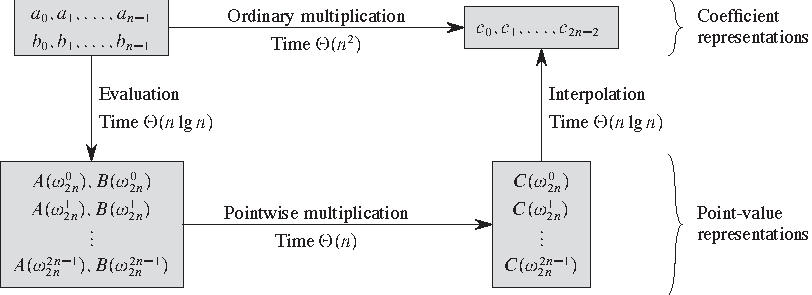
\includegraphics{fft/polynomial-conversion.pdf}
    \caption{Graphical outline of an efficient polynomial multiplication procedure.}
    \label{fig:fft-polynomial-conversion}
\end{figure}

\section{Fast Fourier Transform}

\subsection{Coefficient to Samples (and back)}

Conversion from coefficient to samples is similar to evaluation. We fix a set of points $x_0,x_1,\ldots,x_{n-1}$ and evaluate the polynomial at these points. This evaluation is equivalent to the following matrix multiplication
$$
\mathbf{y} = \mathbf{V} \mathbf{a} =
\begin{bmatrix}
1 & x_0 & x_0^2 & \cdots & x_0^{n-1} \\
1 & x_1 & x_1^2 & \cdots & x_1^{n-1} \\
1 & x_2 & x_2^2 & \cdots & x_2^{n-1} \\
\vdots & \vdots & \vdots & \ddots & \vdots \\
1 & x_{n-1} & x_{n-1}^2 & \cdots & x_{n-1}^{n-1} \\
\end{bmatrix}
\begin{bmatrix} 
    a_0 \\
    a_1 \\
    a_2 \\
    \vdots \\
    a_{n-1}
\end{bmatrix} =
\begin{bmatrix} 
    y_0 \\
    y_1 \\
    y_2 \\
    \vdots \\
    y_{n-1}
\end{bmatrix} 
$$
where $\mathbf{V}$ is called the Vandermonde matrix with entries $V_{jk} = x_j^k$ and $\mathbf{a}$ is the coefficient vector of the polynomial $A(x)$.

Evaluating this matrix product takes $\Theta(n^2)$ scalar operations. Similarly, to convert from samples back to polynomial (interpolation), we can compute $\mathbf{V}^{-1}$ using Gaussian elimination with $O(n^3)$ operations, and computing $\mathbf{a} = \mathbf{V}^{-1}\mathbf{y}$ (it is rarely a good idea to invert any matrices; ``Don't invert that matrix!'' -- John Cook).

In order to obtain efficient algorithms for manipulating polynomials, we need to somehow get rid of the $O(n^2)$ overhead resulted from the interconversion between coefficient and samples.

Note that we simply said ``fix $x_0\ldots x_{n-1}$'' when constructing the Vandermonde matrix without putting any constraints on what values of $x$ to take. By choosing special values for $x$, we can reduce the conversion overhead to $O(n \log n)$.

\subsection{Divide and Conquer}

We can formulate the evaluation $\mathbf{y}=\mathbf{V}\mathbf{a}$ as a divide and conquer algorithm.

We can come up with an outline of the algorithm by following the divide-and-conquer paradigm
\begin{enumerate}
    \item Divide: divide the polynomial $A$ into even and odd coefficients (this is equivalent to divide the coefficient vector $\mathbf{a}$ into even and odd entries)
    $$
    A_{even}(x) = \sum_{k=0}^{\lceil \frac{n}{2}-1 \rceil} a_{2k}x^k \quad \leftrightarrow \quad \mathbf{a}_{even} = \langle a_0,a_2,a_4,\ldots \rangle
    $$
    $$
    A_{odd}(x) = \sum_{k=0}^{\lfloor \frac{n}{2}-1 \rfloor} a_{2k+1}x^k \quad \leftrightarrow \quad \mathbf{a}_{odd} = \langle a_0,a_2,a_4,\ldots \rangle
    $$
    Note that the degree of the two resulting polynomials is half of the original polynomial.

    \item Conquer: recursive conquer $A_{even}(x)$ and $A_{odd}(x)$ for $x \in X^2$ where $X^2 = \{x^2 \mid x \in X\}$.
    
    \item Combine: combine the terms as follows
    $$
    A(x) = A_{even}(x^2) + xA_{odd}(x^2)
    $$
    for $x \in \mathbf{x}$.
\end{enumerate}

It is obvious that the degree of the polynomial $n$ halves, and hence the recurrence
$$
T(n,|X|) = 2T\left( \frac{n}{2},|X| \right) + O(n + |X|) \in O(n^2).
$$
This is no better than the naive approach. The main issue is that we are not halving the size of $X$. Ideally, we want $X$ to be recursively collapsing.

\subsection{Complex Roots of Unity} \index{complex roots of unity}

We can construct a collapsing set of $x$'s via square roots. If we only look at real numbers, taking the square root or squaring a number won't give you fewer or more numbers, but if we broaden our view to complex numbers, we notice that starting from 1, every time we take the square root, the size of the set doubles. The $n$th root of 1 is called the \textbf{complex $n$th root of unity}. The observation implies that if we start from the $n$th root of unity and square the elements in the set, the set will collapse every time we square it.

Example: $\{1\} \to \{1,-1\} \to \{1,-1,i,-i\} \to \{1,-1,i,-i,\pm \frac{\sqrt{2}}{2}(1+i),\pm \frac{\sqrt{2}}{2}(-1+i) \}$

The complex roots of unity are spaced equally around the unit circle centered at the origin of the complex plane. These points are of the form $\cos\theta + i\sin\theta = e^{i\theta}$ for $\theta = 0,\frac{2}{n}\pi,\frac{4}{n}\pi,\ldots,\frac{2(n-1)}{n}\pi$. 

\begin{center}
    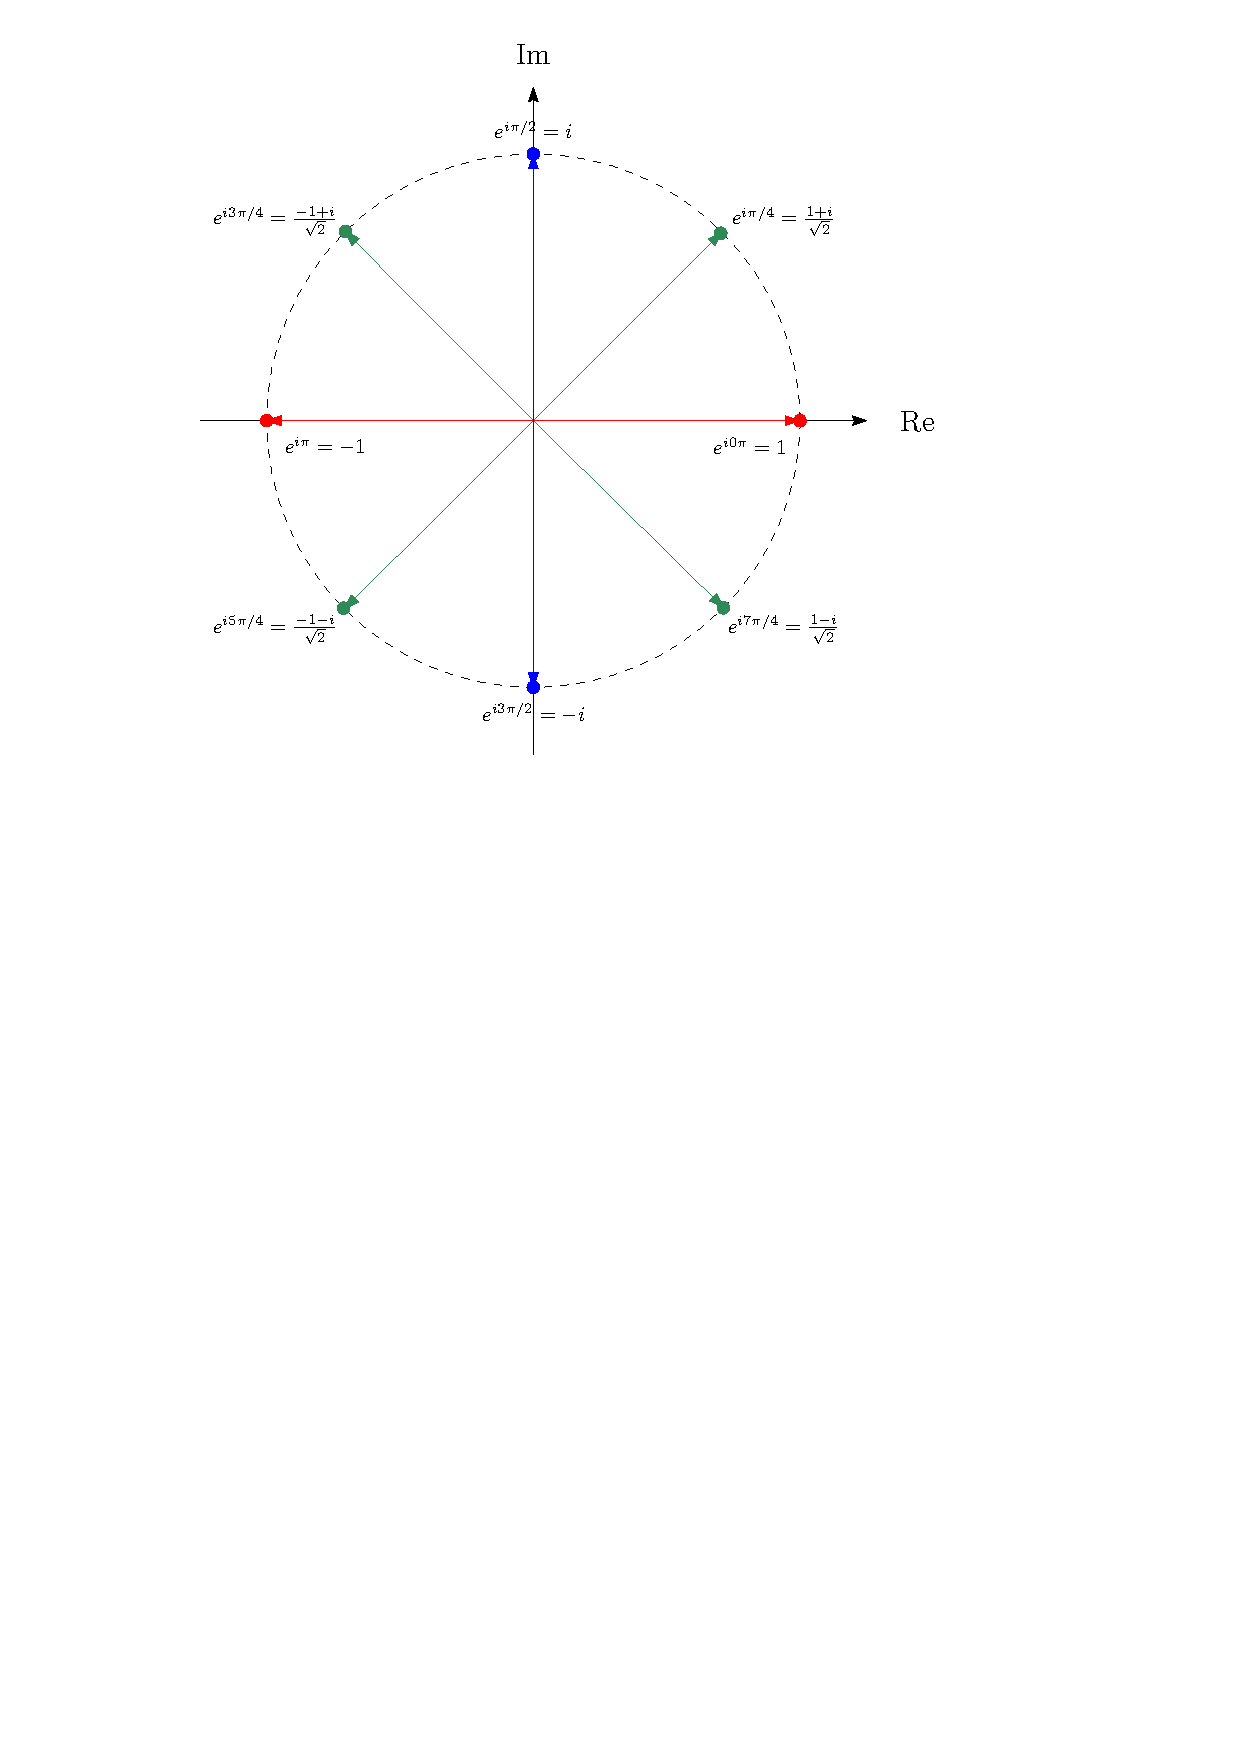
\includegraphics[width=0.6\linewidth]{fft/nth-root-of-unity.pdf}
\end{center}

The $n$th roots of unity where $n=2^\ell$ for some integer $\ell$ form a collapsing set since $(e^{i\theta})^2 = e^{i 2\theta} = e^{i(2\theta \bmod 2\pi)}$. 

Let us formalize this idea and prove that it works.

\begin{lemma}[Halving (Collapsing) Lemma]
    If $n>0$ is even, then the squares of the $n$ complex $n$th roots of unity are the $n/2$ complex $(n/2)$th roots of unity. 
\end{lemma}

\begin{proof}
    We know that $\left(e^{\frac{2\pi i}{n}}\right)^{2k} = e^{\frac{4k\pi i}{n}} = \left(e^{\frac{2\pi i}{1/2 \cdot n}}\right)^k$ for any nonnegative integer $k$. 
    
    Furthermore, $\left(e^{\frac{2\pi i}{n}}\right)^{2(k+n/2)} = \left(e^{\frac{2\pi i}{n}}\right)^{k}$. This implies that for every pair of $k$ and $k+n/2$ share the same square, and that if take the square of every element in the set of $n$th roots of unity, we get the $n/2$ elements and it follows from algebra that the resulting set contains the $(n/2)$th roots of unity.
\end{proof}

\subsection{The FFT Algorithm} \index{fast Fourier transform (FFT)}

By choosing the $x$'s in the Vandermonde matrix to be the $n$th roots of unity, we can make $X$ collapsing along with $n$. The rest of the algorithm is the same as the divide-and-conquer approach described earlier.

\begin{codebox}
    \Procname{$\proc{FFT-Recursive}(a)$}
    \li $n = \attrib{a}{length}$
    \li \If $n \isequal 1$ \Then
        \li \Return $a$ 
    \End
    \li $\omega_n = e^{2\pi i/n}$
    \li $\omega = 1$
    \li $a_{even} = (a_0,a_2,\ldots,a_{n-2})$
    \li $a_{odd} = (a_1,a_3,\ldots,a_{n-1})$
    \li $y_{even} = \proc{FFT-Recursive}(a_{even})$
    \li $y_{odd} = \proc{FFT-Recursive}(a_{odd})$
    \li \For $k = 0$ to $n/2 - 1$ \Do
        \li $y_k = y_{even}[k] + \omega y_{odd}[k]$
        \li $y_{k+\frac{n}{2}} = y_{even}[k] - \omega y_{odd}[k]$
        \li $\omega = \omega \omega_n$
    \End
    \li \Return $y = (y_0,\ldots,y_{n-1})$      
\end{codebox}

This algorithm takes $T(n) = 2T\left( \frac{n}{2} \right) + O(n) \in O(n \log n)$ operations.

\section{Inverse Fast Fourier Transform} \index{inverse fast Fourier transform (IFFT)}

The inverse discrete fourier transform is an algorithm used to find the coefficients fo a polynomial given a set of samples. The transformation is of the form $\mathbf{a}^* \to \mathbf{V}^{-1}\mathbf{a}^* = \mathbf{a}$. To evaluate this, we need $\mathbf{V}^{-1}$. In fact, this matrix has a very useful property that allows to find it without actually inverting $\mathbf{V}$ (again, don't invert the matrix).

\begin{lemma}
    Let $\mathbf{V}$ be the Vandermonde matrix constructed from the set of $n$th roots of unity. Let $\overline{\mathbf{V}}$ denote the complex conjugate of $\mathbf{V}$. Then,
    $$
    \mathbf{V}^{-1} = \frac{1}{n}\overline{\mathbf{V}}
    $$
\end{lemma}

\begin{proof}
    We claim that $\mathbf{P} = \mathbf{V}\overline{\mathbf{V}} = n \mathbf{I}$.

    Let $p_{jk}$ be the $j,k$th entry of $\mathbf{P}$.
    $$
    \begin{aligned}
        p_{jk} &= (\text{row $j$ of $\mathbf{V}$}) \cdot (\text{column $k$ of $\overline{\mathbf{V}}$}) \\
        &= \sum_{m=0}^{n-1} e^{ij2\pi m/n} \overline{e^{ik2\pi m/n}} \\
        &= \sum_{m=0}^{n-1} e^{ij2\pi m/n} e^{-ik2\pi m/n} \\
        &= \sum_{m=0}^{n-1} e^{i(j-k)2\pi m/n}
    \end{aligned}
    $$
    Take $j=k$. Then, $p_{jk} = \sum_{m=0}^{n-1} 1 = n$. Otherwise, $p_{jk} = 0$. This means that the diagonal entries are $n$, and the entires off the diagonal are all 0. Thus, the claim is true.

    It follows that $\mathbf{V}^{-1} = 1/n \mathbf{V}$.
\end{proof}

This lemma implies that for the Inverse Fast Fourier Transform algorithm, we can simply replace $e^{ikr/n}$ with its complex conjugate in the FFT algorithm. The rest of the algorithm is analogous to that for FFT, and it is easy to see that the running of IFFT is also in $O(n \log n)$.

\begin{codebox}
    \Procname{$\proc{IFFT-Recursive}(y)$}
    \li $n = \attrib{y}{length}$
    \li \If $n \isequal 1$ \Then
        \li \Return $y$ 
    \End
    \li $\omega_n = e^{{\color{red}-}2\pi i/n}$
    \li $\omega = 1$
    \li $y_{even} = (y_0,y_2,\ldots,y_{n-2})$
    \li $y_{odd} = (y_1,y_3,\ldots,y_{n-1})$
    \li $a_{even} = \proc{IFFT-Recursive}(y_{even})$
    \li $a_{odd} = \proc{IFFT-Recursive}(y_{odd})$
    \li \For $k = 0$ to $n/2 - 1$ \Do
        \li $a_k = (a_{even}[k] + \omega a_{odd}[k])\; / \;n$
        \li $a_{k+\frac{n}{2}} = (a_{even}[k] - \omega a_{odd}[k])\; / \;n$
        \li $\omega = \omega \omega_n$
    \End
    \li \Return $a = (a_0,\ldots,a_{n-1})$      
\end{codebox}

\section{Fast Polynomial Multiplication}

With FFT, we can implement the procedure outlined in Figure \ref{fig:fft-polynomial-conversion}.

To calculate $A(x)\times B(x)$,

\begin{enumerate}
    \item Compute $A^* = \proc{FFT}(A)$ and $B^* = \proc{FFT}(B)$. This step is $O(n \log n)$.
    \item Compute $C^* = A^* \cdot B^*$ in sample representation. This step is $O(n)$.
    \item Compute $C = \proc{IFFT}(C^*)$ to get $C$ in coefficient representation. This step is $O(n \log n)$.
\end{enumerate}
Overall, the algorithm has runtime complexity of $O(n \log n)$.